\chapter*{}  %加星號隱藏標題

%----------- 重新設定counter格式,章節圖檔和表格的計數器格式皆為1…9 -----------
\renewcommand{\thefigure}{\arabic{chapter}.\arabic{figure}} 
\renewcommand{\thetable}{\arabic{chapter}.\arabic{table}} 
%--------- Input your main figures and tables here  ---------
\setcounter{chapter}{3}%使章節couter切回3,第三章圖放在此行之後
\setcounter{figure}{1}  %使圖檔couter切回1
\setcounter{table}{1}  %使表格couter切回1

\begin{figure}[!]
\centering
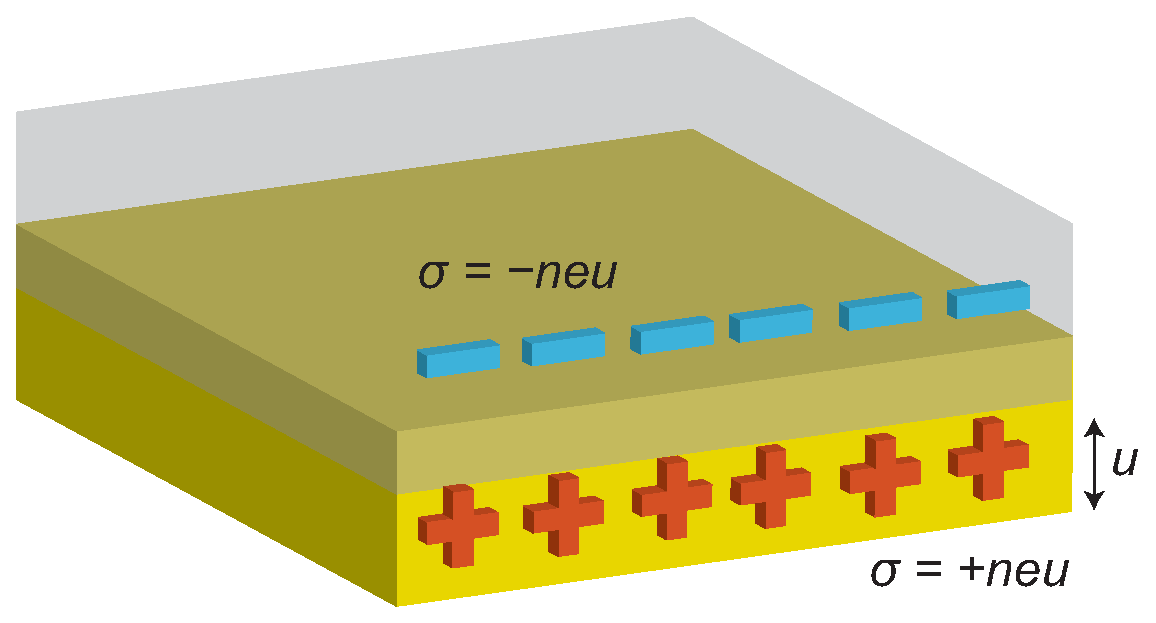
\includegraphics[scale=0.5]{THM/bulk.eps}
\caption{\label{fig:bulk}Longitudinal collective oscillations of the conduction electrons of a metal (Volume plasmons)}
\end{figure}

\begin{table}[!]\begin{center}
\caption{Table Example 1}
\begin{tabularx}{8cm}{llX}
\hline
Start & End  & Character Block Name \\
\hline
3400  & 4DB5 & CJK Unified Ideographs Extension A \\
4E00  & 9FFF & CJK Unified Ideographs \\
\hline
\end{tabularx}
 \end{center}\end{table}
 
\begin{figure}[!]
\centering
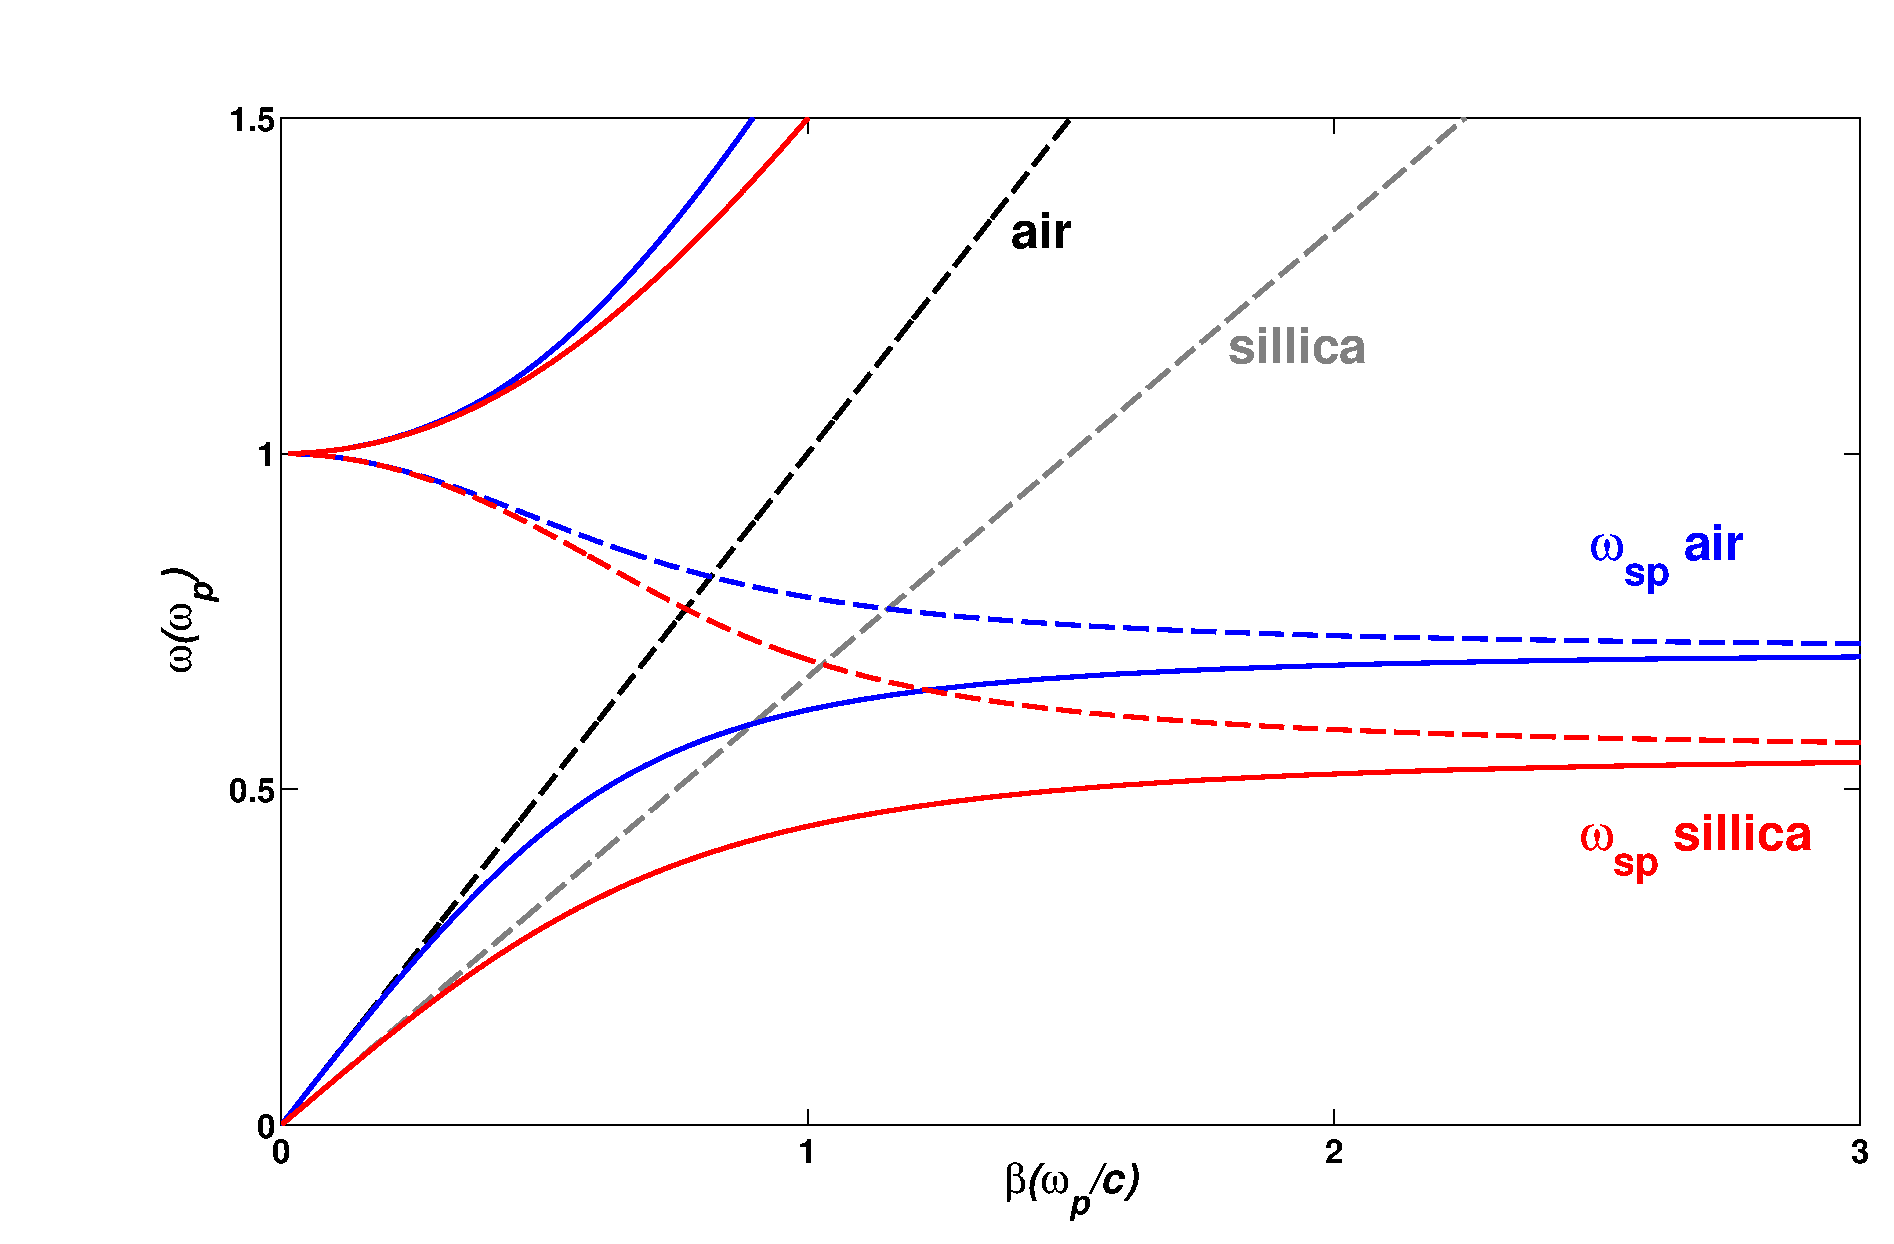
\includegraphics[scale=0.4]{THM/SPPdisp.eps}
\caption{\label{fig:SPPdisp}Dispersion relation of SPPs at the interface between a Drude metal with negligible collision frequency and air (blue curves) and silica (red curves).}
\end{figure}

\setcounter{chapter}{4}  %使章節couter切回4,第4章圖放在此行之後
\setcounter{figure}{1}  %使圖檔couter切回1

\begin{figure}[!]
\centering
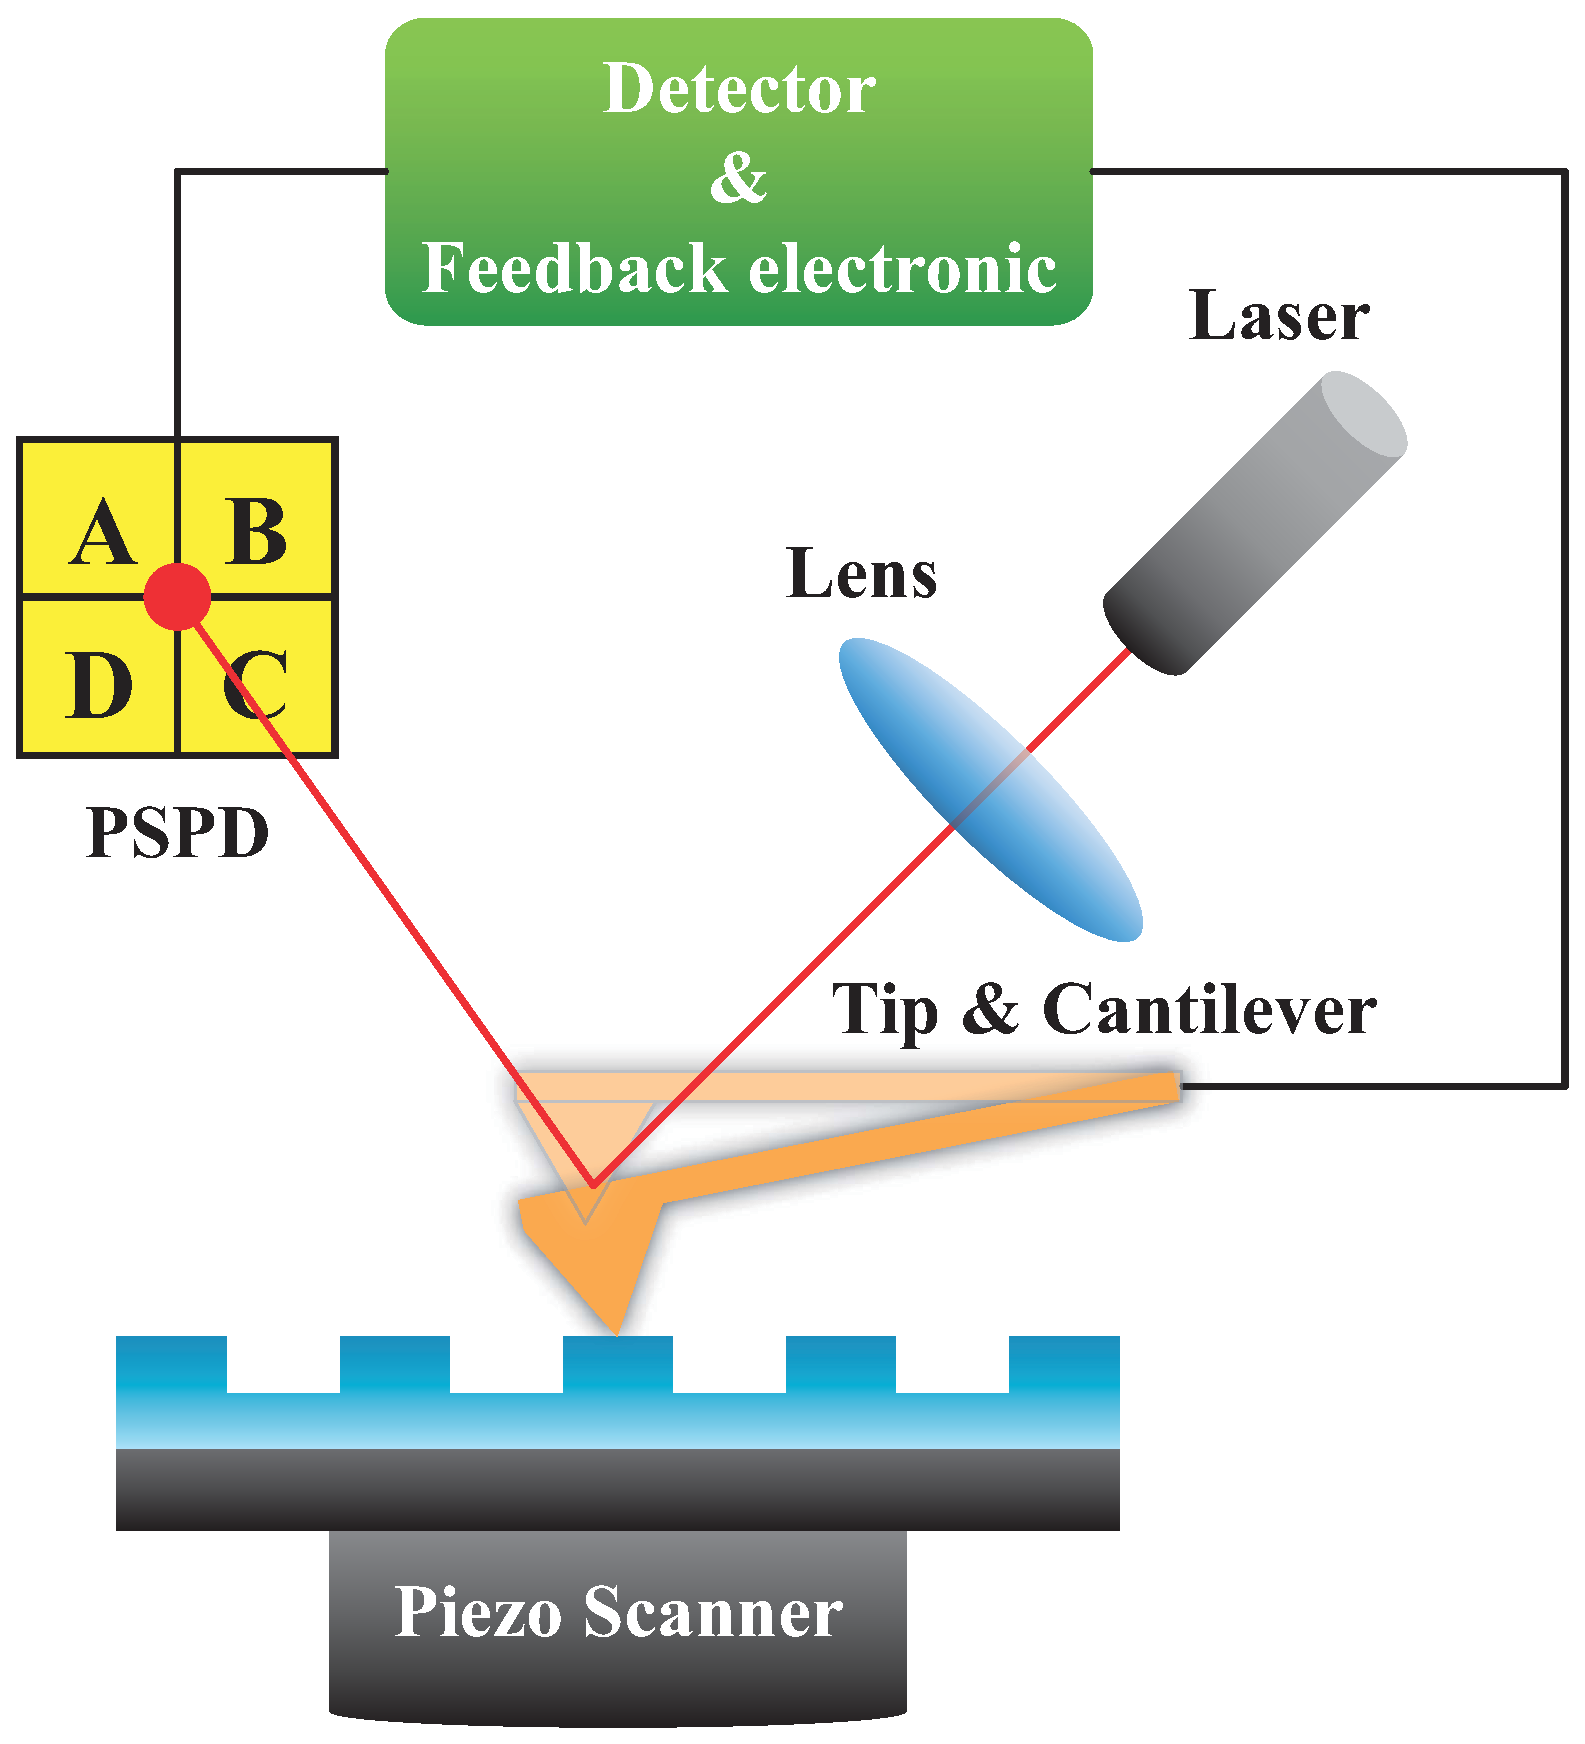
\includegraphics[scale=0.35]{EXP/afm1.eps}
\caption{\label{fig:afm1}Schematic of atomic force microscopy.}
\end{figure}

\begin{figure}[!]
\centering
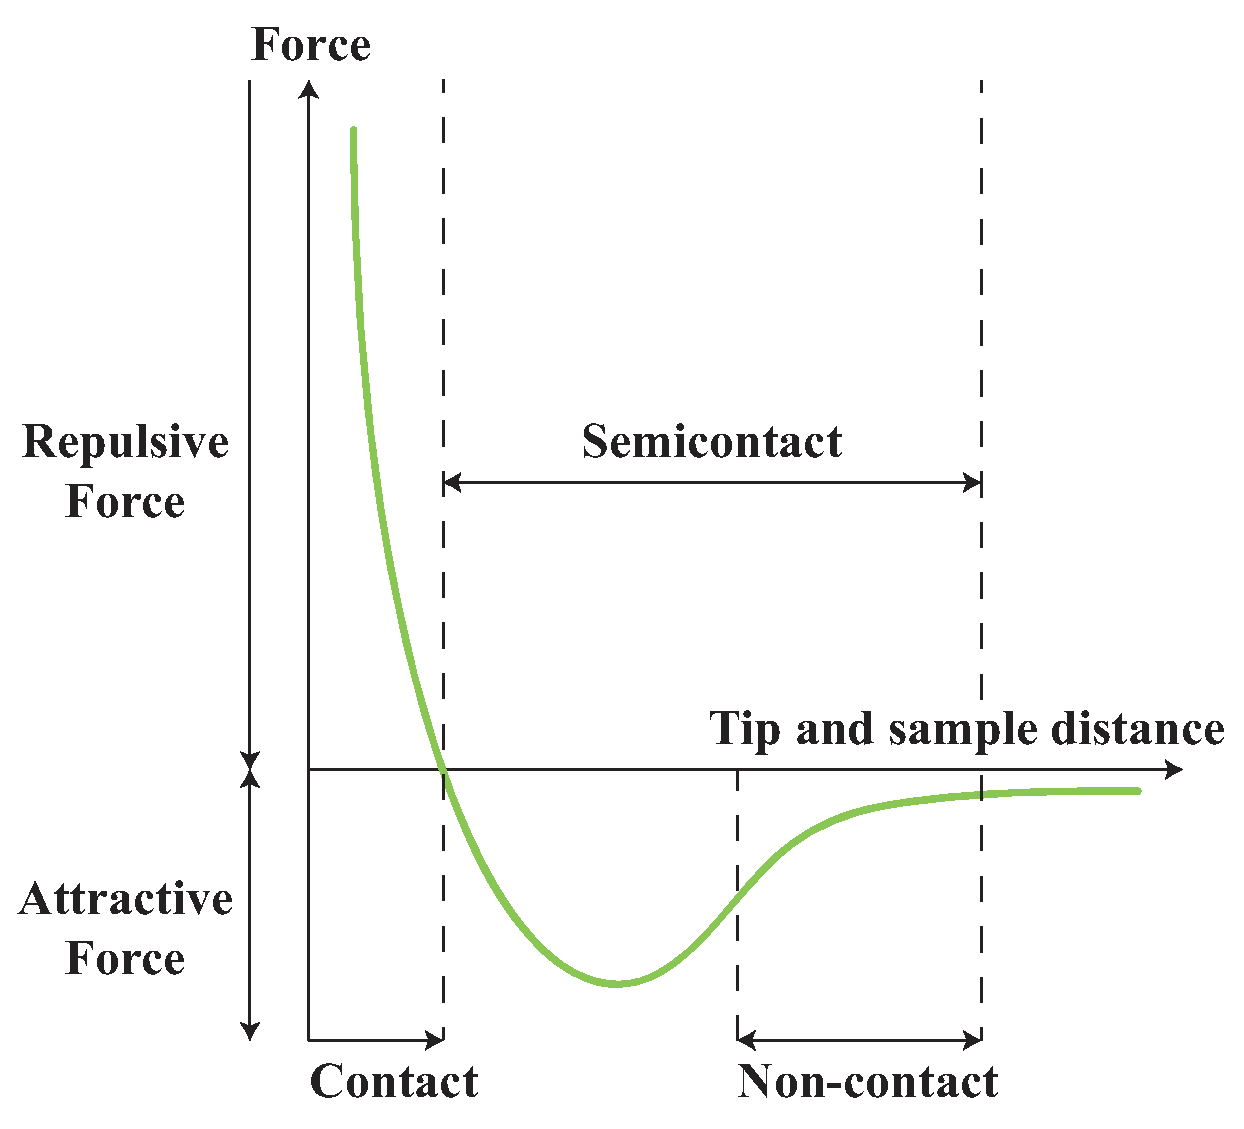
\includegraphics[scale=0.6]{EXP/afm3.eps}
\caption{\label{fig:afm3}Sketch of tip-sample forces.}
\end{figure}

%----------- 重新設定counter格式,章節的計數器格式為A…Z,圖檔和表格的格式皆為1…9 -----------
\renewcommand{\thefigure}{\Alph{chapter}.\arabic{figure}} 
\renewcommand{\thetable}{\Alph{chapter}.\arabic{table}}
%--------- Input your appendix figures and tables here  ---------
\setcounter{chapter}{3}%使章節couter切回3,附錄3圖放在此行之後
\setcounter{figure}{1}  %使圖檔couter切回1
\setcounter{table}{1}  %使表格couter切回1

\begin{figure}[!]
\centering
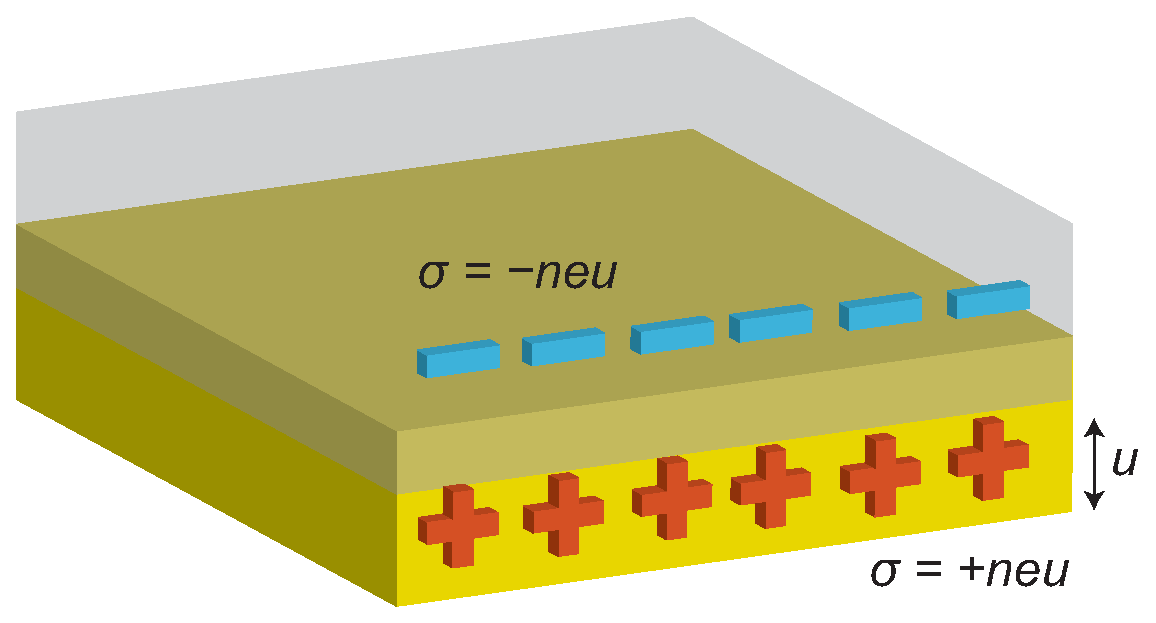
\includegraphics[scale=0.5]{THM/bulk.eps}
\caption{\label{fig:bulk}Longitudinal collective oscillations of the conduction electrons of a metal (Volume plasmons)}
\end{figure}

\begin{table}[!]\begin{center}
\caption{Table Example 1}
\begin{tabularx}{8cm}{llX}
\hline
Start & End  & Character Block Name \\
\hline
3400  & 4DB5 & CJK Unified Ideographs Extension A \\
4E00  & 9FFF & CJK Unified Ideographs \\
\hline
\end{tabularx}
\end{center}\end{table}

\begin{figure}[!]
\centering
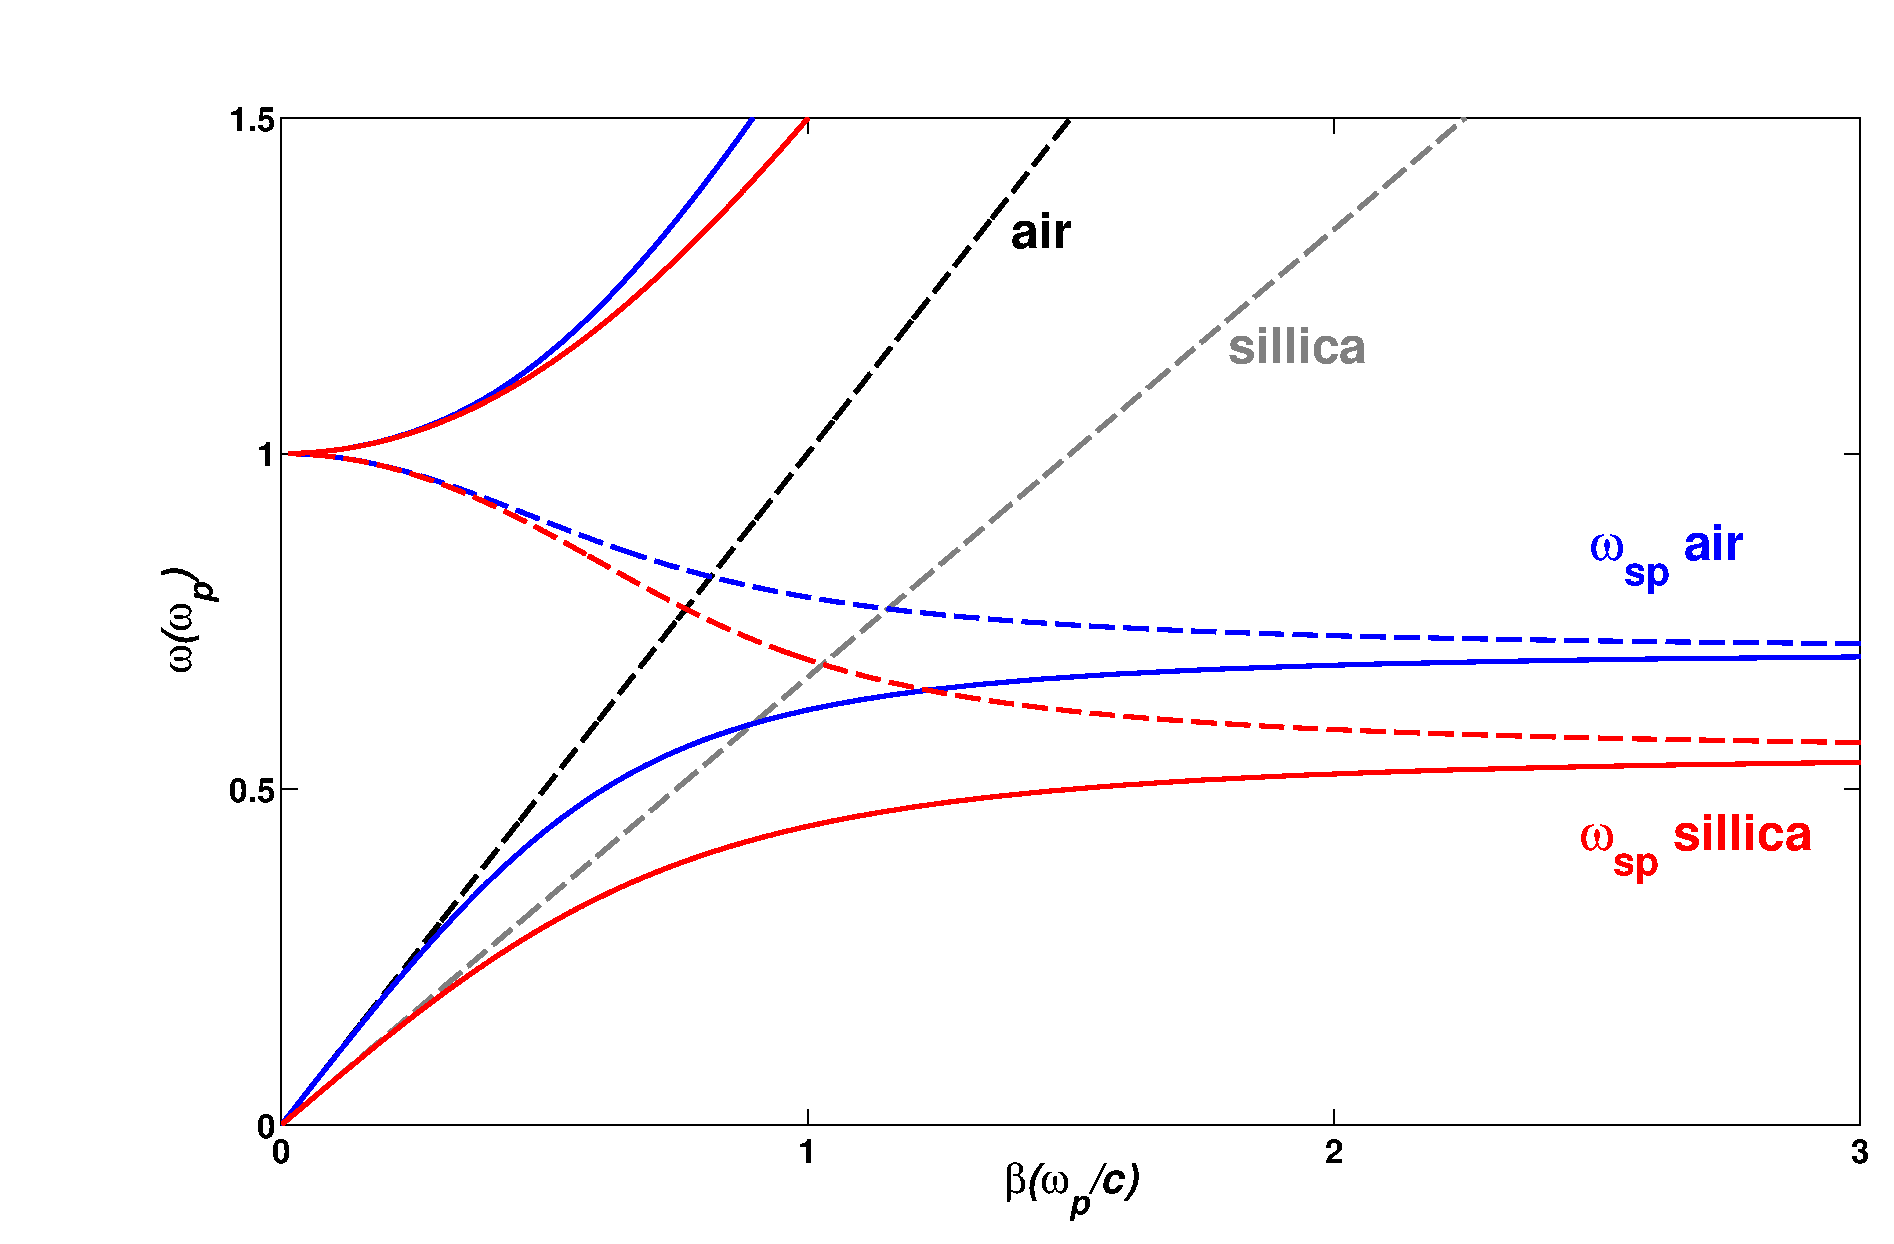
\includegraphics[scale=0.4]{THM/SPPdisp.eps}
\caption{\label{fig:SPPdisp}Dispersion relation of SPPs at the interface between a Drude metal with negligible collision frequency and air (blue curves) and silica (red curves).}
\end{figure}

\setcounter{chapter}{4}  %使章節couter切回4,附錄4章圖放在此行之後
\setcounter{figure}{1}  %使圖檔couter切回1

\begin{figure}[!]
\centering
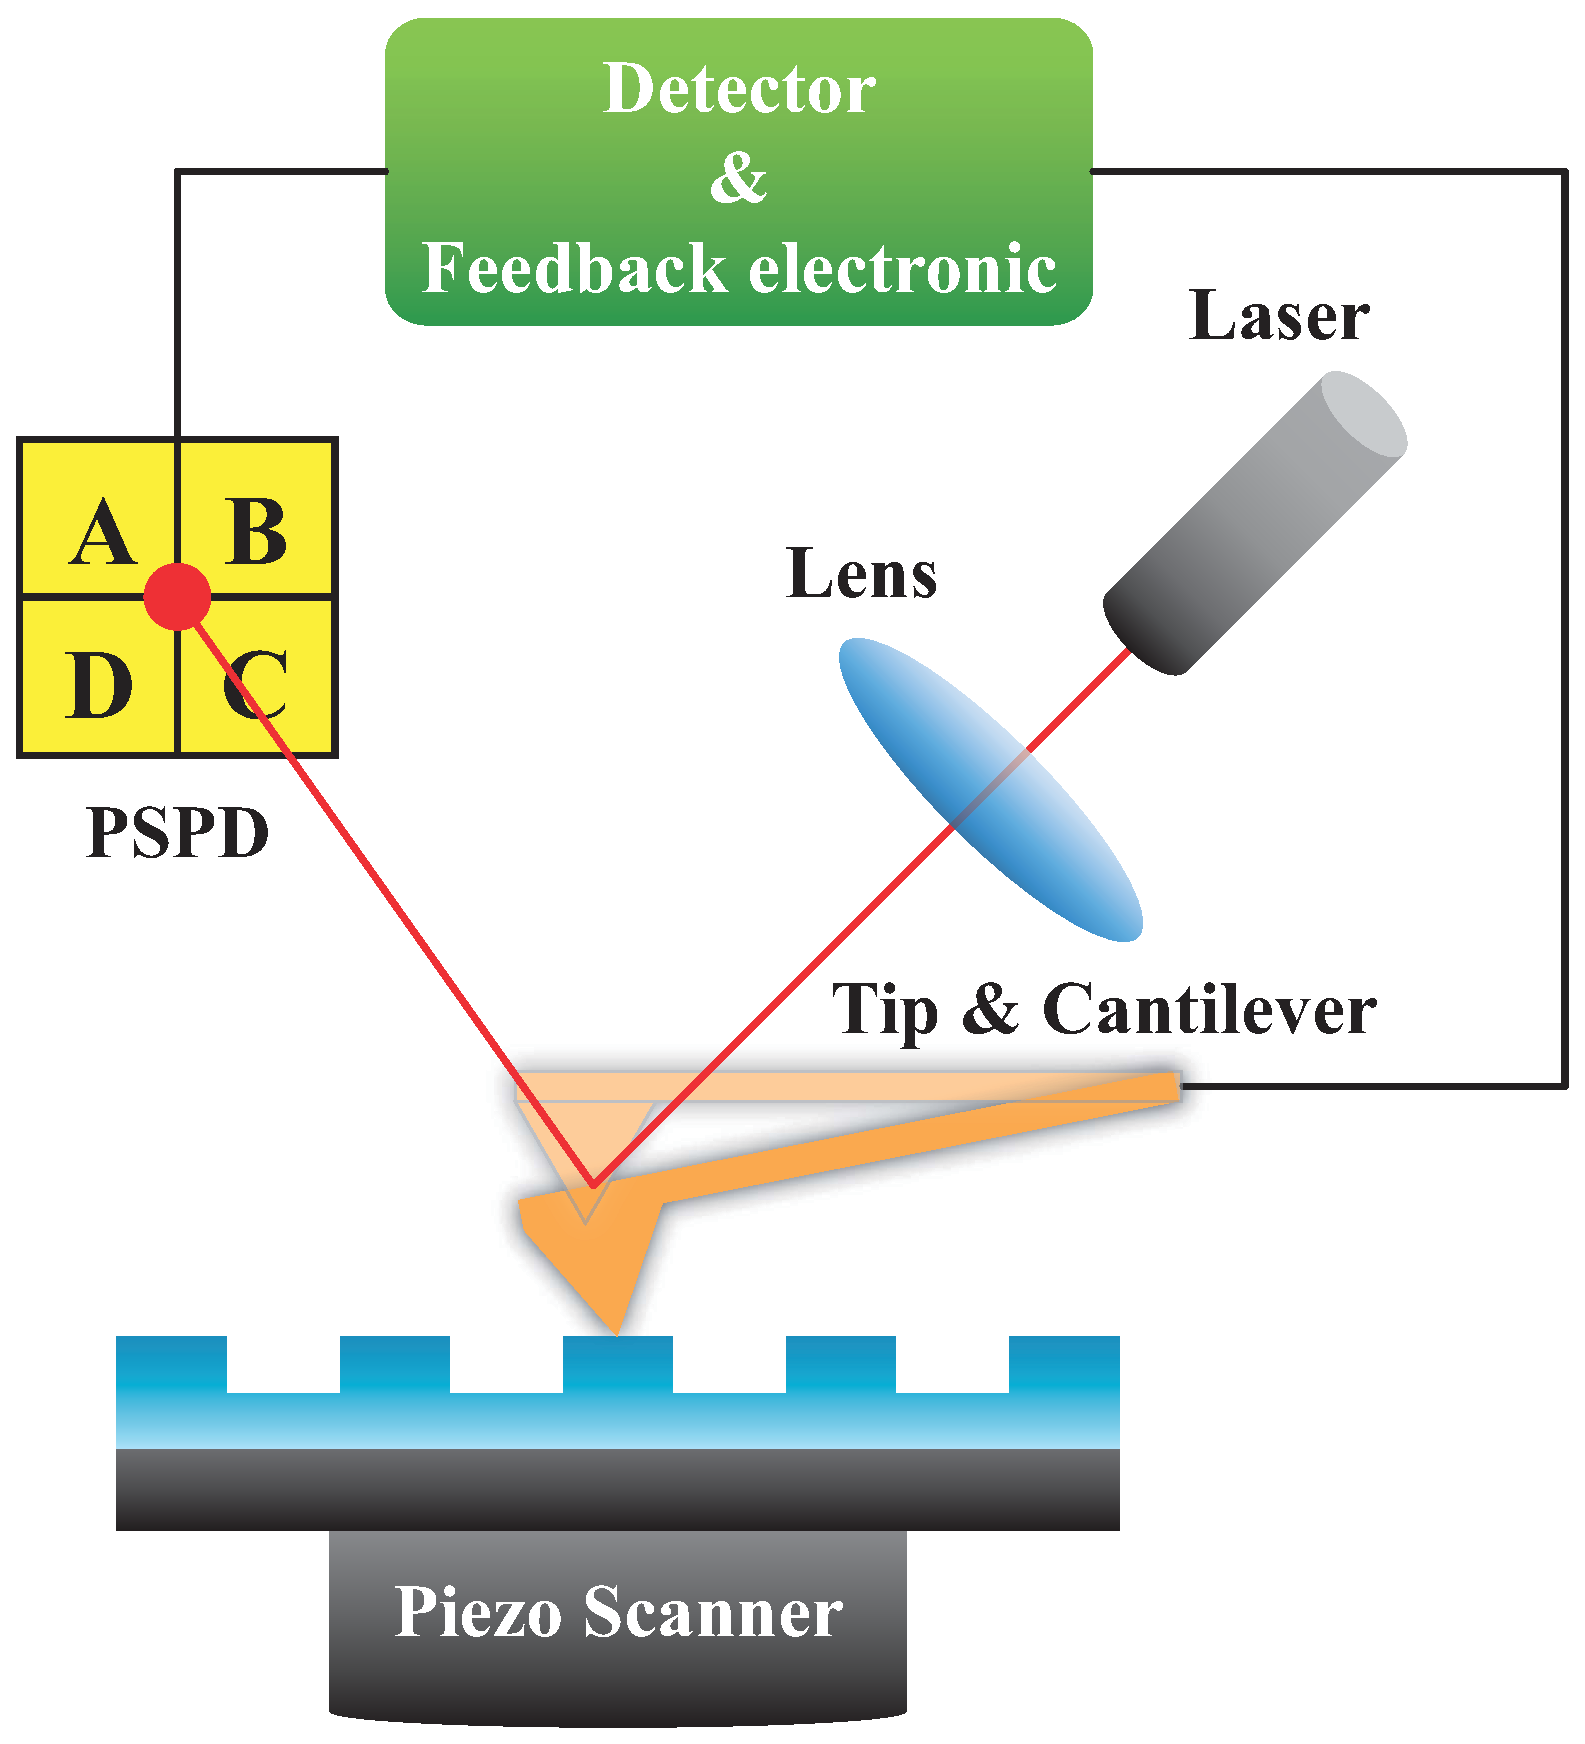
\includegraphics[scale=0.35]{EXP/afm1.eps}
\caption{\label{fig:afm1}Schematic of atomic force microscopy.}
\end{figure}

\begin{figure}[!]
\centering
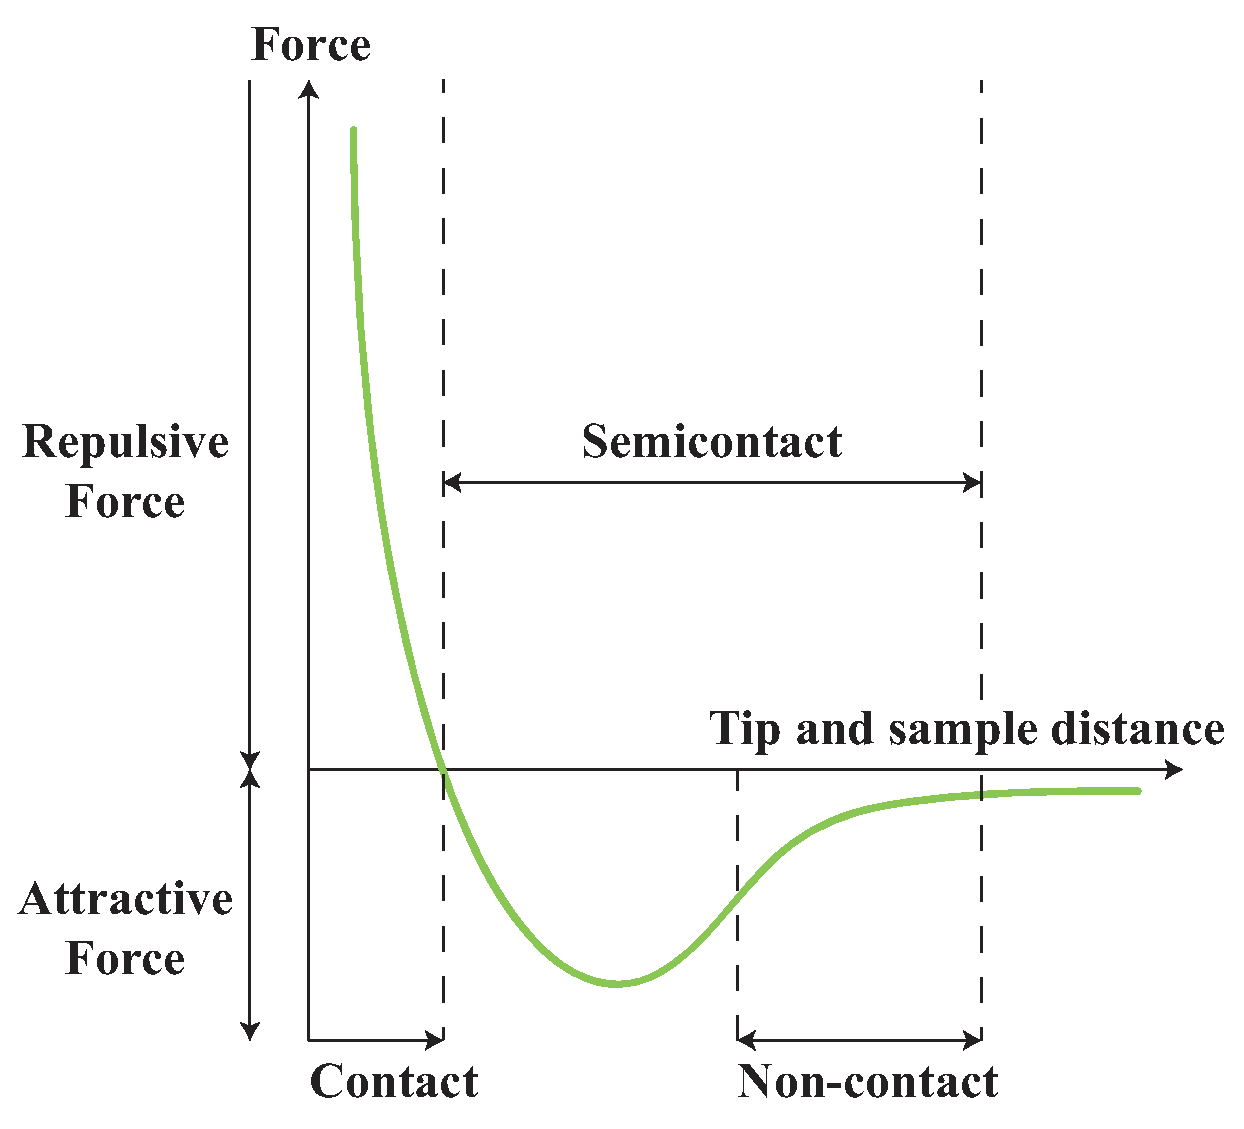
\includegraphics[scale=0.6]{EXP/afm3.eps}
\caption{\label{fig:afm3}Sketch of tip-sample forces.}
\end{figure}